\documentclass[a4paper, 11pt, dvipdfmx]{jsarticle}
\usepackage[utf8]{inputenc}

\usepackage{graphicx}
\usepackage{hyperref}
\usepackage{bookmark}
\usepackage{fontawesome5}
\usepackage{tcolorbox}
\tcbuselibrary{breakable, listingsutf8}

\usepackage{geometry}
\geometry{left=20mm,right=20mm,top=20mm,bottom=20mm}

\usepackage{chngcntr}
\usepackage{listings}
\usepackage{float} % 追加

\tcbset{
  colframe=black,
  colback=gray!20,
  fonttitle=\bfseries\bfseries,
  sharp corners,
  breakable = true,
  boxrule=0.5mm,
  left=1mm,
  right=1mm,
  top=1mm,
  bottom=1mm,
  enlarge top by=1mm, % Adjust the top margin
  enlarge bottom by=1mm, % Adjust the bottom margin
}
\tcbset{
  terminalstyle/.style={
    colframe=black,
    colback=black,
    coltitle=black,
    colbacktitle=white,
    coltext=white,
    fonttitle=\ttfamily,
    rounded corners=north,
    breakable = false,
    title={\faIcon{terminal} terminal},
  },
  yellow/.style={
    colframe=yellow,
    colback=yellow!10,
    coltitle=black,
    fonttitle=\bfseries,
    title={\faIcon{exclamation-triangle} 注意}
  },
  blue/.style={
    colframe=blue,
    colback=blue!10,
    coltitle=white,
    fonttitle=\bfseries,
    title={\faIcon{info-circle} 情報}
  },
  green/.style={
    colframe=green!80!black,
    colback=green!10,
    coltitle=white,
    fonttitle=\bfseries,
    title={\faIcon{bookmark} 補足説明}
  },
}

\newtcolorbox{terminalbox}[1][]{terminalstyle, #1}
\newtcolorbox{commandbox}[2][]{terminalstyle, title={\faIcon{terminal} #2}, #1}
\newtcolorbox{hosokubox}[2][]{green, title={\faIcon{bookmark} #2}, #1}
\newtcolorbox{johobox}[2][]{blue, title={\faIcon{info-circle} #2}, #1}
\newtcolorbox{attentionbox}[2][]{yellow, title={\faIcon{exclamation-triangle} #2}, #1}

\usepackage{titlesec}
\usepackage{tocloft}

% セクション番号の変更
\titleformat{\section}{\normalfont\Large\bfseries}{\thesection 章}{1em}{}
\titleformat{\subsection}{\normalfont\large\bfseries}{\thesection.\arabic{subsection}}{1em}{}
\titleformat{\subsubsection}{\normalfont\normalsize\bfseries}{\thesection.\arabic{subsection}.\arabic{subsubsection}}{1em}{}

\begin{document}

\title{Linuxサーバー構築手順書}
\author{大阪公立大学工業高等専門学校\\
3年 知能情報コース 5番\\
}
\date{\today}
\maketitle\thispagestyle{empty}
\newpage
\tableofcontents

\newpage
\setcounter{section}{-1}

\section{はじめに}

\section{Linuxについて}
\subsection{ファイルやディレクトリ構造について}
Linuxではディレクトリ構造がWindowsとは異なる。
\subsubsection{ファイルの種類}
  Linuxで扱われるファイルは以下のように分類される。
  \begin{itemize}
    \item ファイル     :テキストファイルとバイナリファイル
    \item リンクファイル :シンボリックリンクとハードリンク
    \item 特殊ファイル  :デバイスファイルや隠しファイル
    \item ディレクトリ  :ファイルを集約するためのWindowsでいうフォルダ
  \end{itemize}
  拡張子はWindowsにおいてはアプリケーションの起動に紐づけられていたが、Linuxでは単なるファイル名の一部として認識される。\\
  Linuxではデバイスファイルがあり、これはハードウェアをファイルとして扱うためのものである。\\

  \subsubsection{ディレクトリ構造}
  Linuxのディレクトリ構造は/(ルート)を起点として以下のディレクトリが主に挙げられる。それらをある程度理解しておくことで各種設定などの変更の際に便利である。\\
  \begin{table}[h]
    \centering
    \begin{tabular}{|l|l|}
      \hline
      ディレクトリ & 説明 \\ \hline
      /root & システム管理者のホームディレクトリ \\ \hline
      /home & 一般ユーザーのホームディレクトリ \\ \hline
      /bin & 一般ユーザーでも実行可能なコマンドが含まれるディレクトリ \\ \hline
      /sbin & sudo権限またはroot権限が必要なコマンドが含まれるディレクトリ \\ \hline
      /media & USBメモリや外付けHDDなどのデバイスがマウントされるディレクトリ \\ \hline
      /etc & システムの設定ファイルが含まれるディレクトリ \\ \hline
      /usr & システム全体で共有されるアプリケーション、ライブラリ、ドキュメントなどが保存されるディレクトリ \\ \hline
      /lib & ライブラリが保存されるディレクトリ \\ \hline
      /proc & カーネルやプロセスに関する情報が保存されるディレクトリ \\ \hline
      /tmp & 一時ファイルが保存されるディレクトリ \\ \hline
      /var & 変化するデータが保存されるディレクトリ、ログファイルやデータベースなど \\ \hline
    \end{tabular}
    \caption{主要なディレクトリとその説明}
    \label{tab:directories}
  \end{table}
  表\ref{tab:directories}に主要なディレクトリとその説明を示す。


\section{Ubuntuインストール}
\subsection{インストールメディアの準備}
  \begin{enumerate}
    \item UbuntuのISOファイルをダウンロード
    \begin{tcolorbox}[blue]
      Ubuntu を入手する \href{https://releases.ubuntu.com/20.04/}{\texttt{https://releases.ubuntu.com/20.04/}}\\
      Ubuntu Desktop 日本語 Remixのダウンロード \href{https://www.ubuntulinux.jp/download/ja-remix}{\texttt{https://www.ubuntulinux.jp/download/ja-remix}}
    \end{tcolorbox}
    \item Rufusをダウンロード
    \begin{tcolorbox}[blue]
      Rufusを入手する \href{https://rufus.ie/ja/}{\texttt{https://rufus.ie/ja/}}
    \end{tcolorbox}
    \item Rufusを起動し、デバイス、ブート選択、イメージ選択を行う\\
    デバイスにはインストールメディアとするためのUSBを選択する。\\
    ブート選択では、先ほどダウンロードしたISOファイルを選択する。\\
    パーティション構成は一般的にはMBRでよい。ただし、Gatewayの場合はGPTを選択する。その他の設定はデフォルトのままでよい。
      \begin{tcolorbox}[yellow]
        デバイスを選択する際は注意が必要である。間違えるとPCや外部ストレージのデータが消える可能性があるため、注意が必要である。
      \end{tcolorbox}
    \item スタートをクリックし、書き込みを開始する
  \end{enumerate}

\subsection{Boot Modeの変更}
  \begin{enumerate}
    \item 電源をつけF2を連打しBIOS画面を表示
    \item Securityに移動しSupervisor Passwordを設定
    \item Bootに移動しBoot ModeをLegacyに変更
    \item F10で保存して再起動
    \item F2を連打しBIOS画面を表示
    \item Bootに移動しBoot Priorityを変更しインストールメディアが入るものを選択
    \item Boot ModeをUEFIに変更
    \item SecureBootをDisableに変更
    \item F10で保存して再起動
  \end{enumerate}
\subsection{Ubuntuのインストール}
  \begin{enumerate}
    \item 再起動後自動的にBoot Menuが表示される
    \item Try or Install Ubuntuを選択
    % \item 以下Ubuntuのインストールを書く ★
    \item インストールの種類を選択
    \item インストール先を選択
    \item キーボードレイアウトを選択
    \item ユーザー情報を入力
    \item インストールが完了したら再起動
  \end{enumerate}
\subsection{インストール後の再起動}
  \begin{enumerate}
    \item 再起動時にBiosに入る
    \item Bootに移動しBoot Priorityを変更しインストールしたディスクを1番目にする
    \item SecureをEnableに変更
    \item Securityに移動しErase all Secure Boot Settingを選択し、Boot設定を削除
    \item Select an UEFI file as trusted for executingを選択
    \item EMMC \textgreater EFI \textgreater Ubuntu \textgreater shimx64.efiを選択
    \item Boot名を入力し、Enter
    \item Bootに移動しSecure BootをDisableに変更
    \item Securityに移動しSupervisor Passwordを削除
    \item F10で保存して再起動
    \item ログイン画面になったら成功
  \end{enumerate}

\section{Ubuntuの各種設定・インストール}
Ubuntu(Linux)はWindowsなどと同様に様々な設定が可能である。以下にはその一部を示すが、適宜自分にあったUbuntu環境を構築することが望ましい。練習ついでにいろいろな物を入れてみるとよい。
\subsection{日本語入力}
  Ubuntuではデフォルトでキーボードによる日本語入力は対応していない。そのため、以下の手順で日本語入力を可能にする。なお日本語入力には一般に「Mozc」が使用されることが多い。
  \begin{enumerate}
    \item ターミナルを開く
    \item 以下のコマンドを実行
    \begin{terminalbox}
      \verb|$ sudo apt update|\\
      \verb|$ sudo apt install ibus-mozc|
    \end{terminalbox}
    \item 設定 \textgreater キーボード \textgreater 入力ソース \textgreater 日本語(Mozc)を追加
    \item Windowsキー + Spaceで日本語入力が可能になる\\
    なお、右上にある「A」をクリックすることで入力ソースを切り替えることができる。
  \end{enumerate}

\subsection{Vimのインストール}
  VimはLinux環境で使用されるテキストエディタであり、非常に高機能である。特徴として、ターミナル上で操作するため、マウスを使わずに編集を行う。本手手順書ではsudo権限(後の章にて解説)の必要なファイルの編集などで使用する。標準で搭載されている場合もある。
  \begin{enumerate}
    \item ターミナルを開く
    \item 以下のコマンドを実行
    \begin{terminalbox}
      \verb|$ sudo apt update|\\
      \verb|$ sudo apt install vim|
    \end{terminalbox}
    \item インストールが完了したら、以下コマンドを実行しインストールされているか確認
    \begin{terminalbox}
      \verb|$ vim --version|
    \end{terminalbox}
  \end{enumerate}

\subsection{VSCodeのインストール}
  VSCodeはMicrosoftが提供するオープンソースのコードエディタであり、非常に高機能である。特徴として、拡張機能を追加することで、様々な言語に対応することができる。また、リモート開発機能を使用することで、リモートサーバー上での開発も可能である。
  \begin{enumerate}
    \item \href{https://code.visualstudio.com/}{\texttt{https://code.visualstudio.com/}}にアクセスし、ダウンロード
    \item ダウンロードしたファイルを開く
    \item インストールを開始
    \item インストールが完了したら、VSCodeを起動
  \end{enumerate}

\subsection{slのインストール(お遊び)} 
  slは、タイプミスでよく入力される「ls」コマンドを実行すると、蒸気機関車が走るアニメーションが表示されるコマンドである。インストールの練習として入れてみるとよい。
  \begin{enumerate}
    \item ターミナルを開く
    \item 以下のコマンドを実行
    \begin{terminalbox}
      \verb|$ sudo apt update|\\
      \verb|$ sudo apt install sl|
    \end{terminalbox}
    \item 以下のコマンドを実行
    \begin{terminalbox}
      \verb|$ sl|
    \end{terminalbox}
  \end{enumerate}
  \begin{figure}[H]
    \centering
    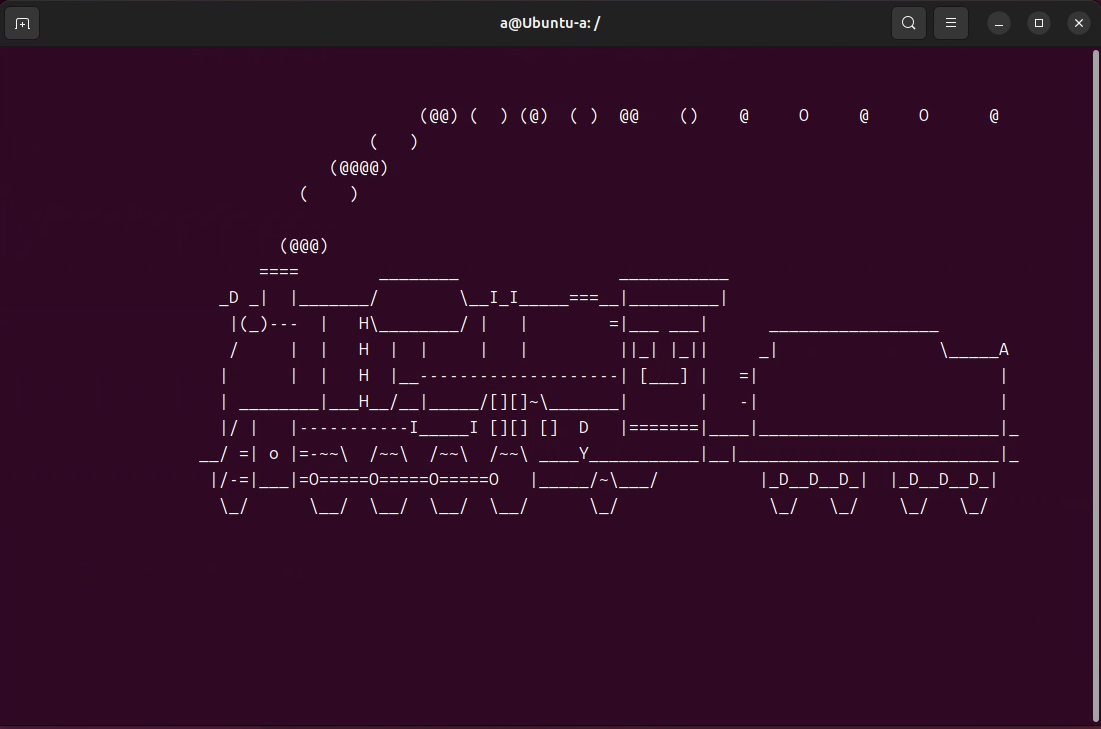
\includegraphics[width=0.5\textwidth]{images/linux-server/3_4-sl.png}
    \caption{slの実行結果}
    \label{fig:sl}
  \end{figure}
  実行時にオプションがあるので、気が向いたら調べて遊んでみるとよい。

\subsection{cmatrixのインストール(お遊び)}
  cmatrixは、映画「マトリックス」に登場するコードのような文字列が画面上を流れるアニメーションを表示するコマンドである。ハッカーみたいになれるのでなりたい人は入れるとよい。
  \begin{enumerate}
    \item ターミナルを開く
    \item 以下のコマンドを実行
    \begin{terminalbox}
      \verb|$ sudo apt update|\\
      \verb|$ sudo apt install cmatrix|
    \end{terminalbox}
    \item 以下のコマンドを実行
    \begin{terminalbox}
      \verb|$ cmatrix|
    \end{terminalbox}
  \end{enumerate}
  \begin{figure}[H]
    \centering
    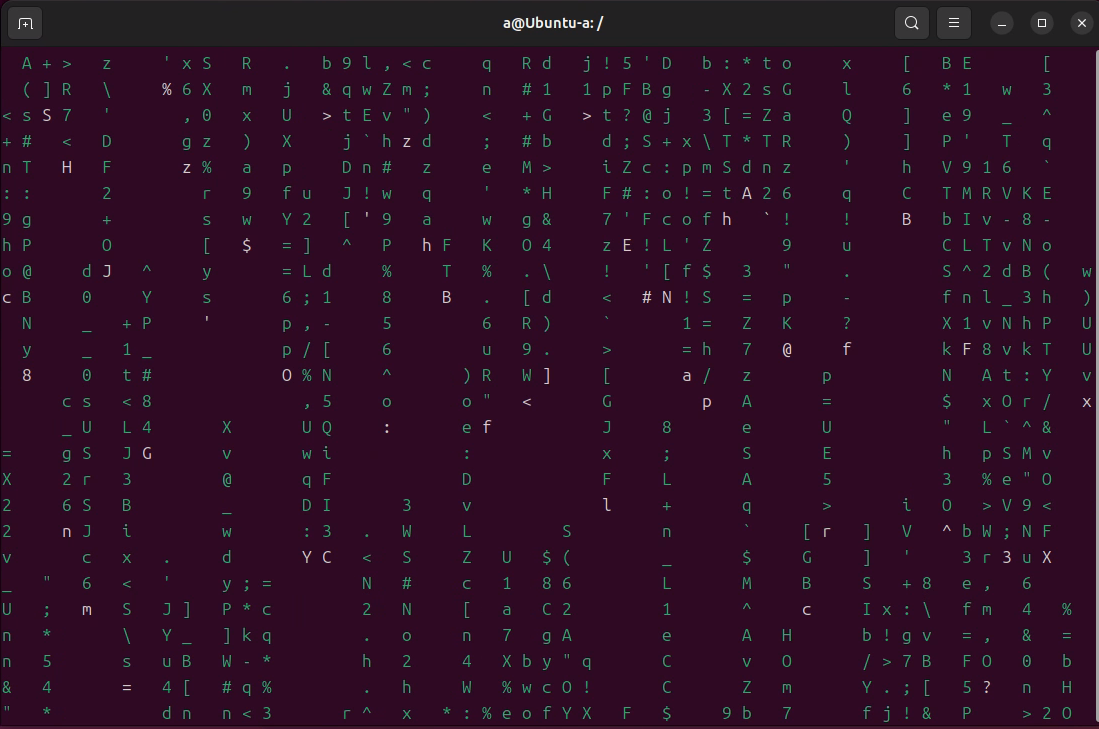
\includegraphics[width=0.5\textwidth]{images/linux-server/3_5-cmatrix.png}
    \caption{cmatrixの実行結果}
    \label{fig:cmatrix}
  \end{figure}

\section{Linuxの基本コマンド}
サーバー上でのシステム操作は一般的にターミナルを用いてコマンド入力により操作を行うことが多い。この章ではLinuxの基本コマンドとして紹介するが、一部コマンドはWindowsでも使用できる。ただし、WindowsのコマンドはLinuxとは異なるため注意が必要である。\\
  コマンドは一般的に以下のように入力する。
\begin{commandbox}{コマンドの入力方法}
  \verb|$ {コマンド名} {オプション} {引数}|
\end{commandbox}

\subsection{よく使うコマンド一覧}
\subsubsection{ファイルやディレクトリの操作}
\begin{itemize}
  \item ls : ファイルやディレクトリの一覧を表示する\\
  オプションなしの場合、カレントディレクトリのファイルやディレクトリの一覧を表示する。
  \begin{terminalbox}
    \verb|$ ls|
    \verb|bin |
  \end{terminalbox}
  \begin{hosokubox}{lsコマンドのオプション}
    -a : 隠しファイルも表示する\\
    -l : 詳細情報を表示する(パーミッション情報)\\
    -h : ファイルサイズを見やすい形式で表示する
  \end{hosokubox}
  \item cd : カレントディレクトリを移動する\\
  ディレクトリ名の場所にカレントディレクトリを移動する。
  \begin{terminalbox}
    \verb|$ cd {ディレクトリ名}|\\\\
    \verb|# ルートディレクトリへの移動|\\
    \verb|$ cd /|
  \end{terminalbox}
  \item pwd : 現在のディレクトリのパスを表示する
  \begin{terminalbox}
    \verb|$ pwd|\\\\
    \verb|例:/homeでの実行結果|\\
    \verb|/home|
  \end{terminalbox}
  \item mkdir : ディレクトリを作成する\\
  pathに指定したディレクトリを作成する。
  \begin{terminalbox}
    \verb|$ mkdir {ディレクトリ名}|\\\\
    \verb|例:testディレクトリを作成する|\\
    \verb|$ mkdir test|
  \end{terminalbox}
  \item rm : ファイルやディレクトリを削除する\\
  一部ファイルはsudo権限が必要である。
  \begin{terminalbox}
    \verb|$ rm {ファイル名}|\\\\
    \verb|例:test.txtを削除する|\\
    \verb|$ rm test.txt|
  \end{terminalbox}
  \item rmdir : ディレクトリを削除する\\
  ディレクトリ内にファイルがある場合は削除できない。
  \begin{terminalbox}
    \verb|$ rmdir {ディレクトリ名}|\\\\
    \verb|例:testディレクトリを削除する|\\
    \verb|$ rmdir test|
  \end{terminalbox}
  \item cp : ファイルやディレクトリをコピーする\\
  copyであるため元のファイルは残る。
  \begin{terminalbox}
    \verb|$ cp {コピー元} {コピー先}|\\\\
    \verb|例:test.txtをtest2.txtにコピーする|\\
    \verb|$ cp test.txt test2.txt|
  \end{terminalbox}
  \item mv : ファイルやディレクトリを移動する\\
  moveであるため元のファイルは消える。
  \begin{terminalbox}
    \verb|$ mv {移動元} {移動先}|\\\\
    \verb|例:test.txtをtest2.txtに移動する|\\
    \verb|$ mv test.txt test2.txt|
  \end{terminalbox}
  \item find : ファイルを検索する
  \begin{terminalbox}
    \verb|$ find {検索先} -name {検索ファイル名}|
  \end{terminalbox}
  \item touch : ファイルを作成する
  \begin{terminalbox}
    \verb|$ touch {ファイル名}|\\\\
    \verb|例:test.txtファイルを作成する|\\
    \verb|$ touch test.txt|
  \end{terminalbox}
  \item ln:シンボリックリンクの作成\\
  ファイルやディレクトリに対してシンボリックリンクを作成する。シンボリックリンクとはWindowsにおけるショートカットの役割を果たすものである。
  \begin{terminalbox}
    \verb|$ ln -s {リンク元} {リンク先}|\\\\
    \verb|例:test.txtのシンボリックリンクをデスクトップに作成する|\\
    \verb|$ ln -s test.txt ~/Desktop/test.txt|
  \end{terminalbox}
\end{itemize}

\subsubsection{テキスト操作}
\begin{itemize}
  \item cat : ファイルの内容を表示する\\
  ファイルの内容をターミナル上でスクロールする形で表示する。
  \begin{terminalbox}
    \verb|$ cat {ファイル名}|
  \end{terminalbox}
  \item less : ファイルの内容をページ単位で表示する
  スペースキーで次のページ、qキーで終了する。
  \begin{terminalbox}
    \verb|$ less {ファイル名}|
  \end{terminalbox}
  \item head : ファイルの先頭部分を表示する\\
  ファイルの先頭部分を表示する。
  \begin{terminalbox}
    \verb|$ head {ファイル名}|
  \end{terminalbox}
  \item tail : ファイルの末尾部分を表示する\\
  ファイルの末尾部分を表示する。
  \begin{terminalbox}
    \verb|$ tail {ファイル名}|
  \end{terminalbox}
  \item grep : ファイル内の文字列を検索する\\
  ファイル内の文字列を検索する。
  \begin{terminalbox}
    \verb|$ grep {検索文字列} {ファイル名}|\\\\
    \verb|例:test.txt内に「test」が含まれているか検索する|\\
    \verb|$ grep test test.txt|
  \end{terminalbox}
  \item vi : Vim(テキストエディタ)の起動\\
  Vimの使用方法については後述する。
  \begin{terminalbox}
    \verb|$ vi {ファイル名}|\\\\
    \verb|例:test.txtを編集する|\\
    \verb|$ vi test.txt|
  \end{terminalbox}
  \item code : VSCode(テキストエディタ)の起動\\
  ファイル名の部分にはディレクトリも指定できる。その場合、そのディレクトリがVSCodeで開かれる。
  \begin{terminalbox}
    \verb|$ code {ファイル名}|\\\\
    \verb|例:test.txtを編集する|\\
    \verb|$ code test.txt|
  \end{terminalbox}
\end{itemize}

\subsubsection{パーミッションや所有者}
\begin{itemize}
  \item chmod : ファイルやディレクトリのパーミッションを変更する\\
  \begin{terminalbox}
    \verb|$ chmod {パーミッション} {ファイル名}|\\\\
    \verb|例:test.txtのパーミッションをrwxr-xr--に変更する|\\
    \verb|$ chmod 754 test.txt|
  \end{terminalbox}
  パーミッションはrwxrwxrwxの形式で表される。rは読み取り、wは書き込み、xは実行を表す。\\
  例えば、rwxr-xr--は所有者に読み取り、書き込み、実行権限があり、グループに読み取り、実行権限があり、その他に読み取り権限があることを示す。
  \begin{hosokubox}{パーミッションの指定方法について}
    パーミッションは数字で指定することができる。\\
    rwx/rwx/rwxという風に3桁ごとに区切って考える。rを4, wを2, xを1として、それぞれの権限を足し合わせる。したがって、rwxr-xr--は754と表すことができる。\\
    ※この数字は2進数で処理しており、rwxの時111となり、合計が7となる。
  \end{hosokubox}
  \item chown : ファイルやディレクトリの所有者を変更する
  \begin{terminalbox}
    \verb|$ chown {所有者}:{グループ} {ファイル名}|\\\\
    \verb|例:test.txtの所有者をrootに変更する|\\
    \verb|$ chown root test.txt|
  \end{terminalbox}
  グループ名は省略することもできる。その場合、所有者と同じグループになる。
  \item chgrp : ファイルやディレクトリのグループを変更する
  \begin{terminalbox}
    \verb|$ chgrp {グループ} {ファイル名}|\\\\
    \verb|例:test.txtのグループをrootに変更する|\\
    \verb|$ chgrp root test.txt|
  \end{terminalbox}
\end{itemize}

\subsubsection{ネットワーク管理}
\begin{itemize}
  \item ping : ネットワークの接続確認を行う
  \begin{terminalbox}
    \verb|$ ping {IPアドレス}|\\\\
    \verb|例:192.168.0.150にpingを送信する|\\
    \verb|$ ping 192.168.0.150|
  \end{terminalbox}
  \begin{hosokubox}{pingコマンドについて}
    pingコマンドはネットワーク内の機器の接続確認でよく使用される。Windowsでも同様に使用できる。ただし、Windowsは4回の送信で終了するが、LinuxはCtrl + Cで終了するまで続く。
  \end{hosokubox}
  \begin{hosokubox}{pingコマンドのオプション}
    -c : 指定回数の送信を行う\\
    -i : 送信間隔を指定する\\
    -t : 継続的に送信を行う
  \end{hosokubox}
  \item ifconfig : ネットワークインターフェースの情報を表示する
  \begin{terminalbox}
    \verb|$ ifconfig|
  \end{terminalbox}
  出力例は以下の通りである。
  \begin{figure}[H]
    \centering
    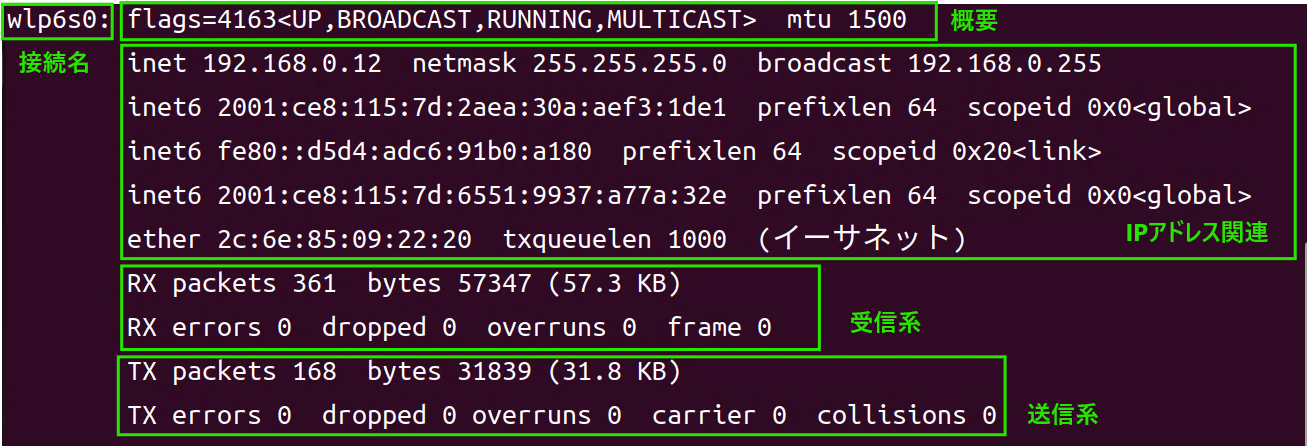
\includegraphics[width=0.8\textwidth]{images/linux-server/4_1_4-1-ifconfig.png}
    \caption{ifconfigの出力例}
    \label{fig:your_image}
  \end{figure}
  各種いろいろなネットワークアダプタに関する情報を取得できるがため調べて利用するとよい。ただし、IPアドレス関連にあるinetアドレスは、IPv4のアドレスでありよく使うため覚えておくとよい。
  \item route : ルーティングテーブルの情報を表示する
  \begin{johobox}{ルーティングとは}
    ルーティングとは、ネットワーク上のデータを送信する際に、どの経路を通って送信するかを決定することである。ルーティングテーブルは、どの経路を通って送信するかを示すものである。
  \end{johobox}
  \begin{terminalbox}
    \verb|$ route|
  \end{terminalbox}
  \item netstat : ネットワークの接続状況を表示する
  \begin{terminalbox}
    \verb|$ netstat|\\\\
    \verb|例:全ての接続状況を表示する|\\
    \verb|$ netstat -a|
  \end{terminalbox}
  \begin{hosokubox}{netstatコマンドのオプション}
    -a : 全ての接続状況を表示する\\
    -t : TCP接続のみを表示する\\
    -u : UDP接続のみを表示する\\
    -n : IPアドレスを表示する
  \end{hosokubox}
  \item ssh : リモートサーバーに接続する\\
  詳細については10章で解説する。
  \begin{terminalbox}
    \verb|$ ssh {ユーザー名}@{IPアドレス}|
  \end{terminalbox}
  \item ftp : ファイル転送プロトコルを使用してファイルを転送する
  \begin{terminalbox}
    \verb|$ ftp {IPアドレス}|
  \end{terminalbox}
\end{itemize}

\subsubsection{システム管理}
\begin{itemize}
  \item top : システムのリソース使用状況を表示する
  \begin{terminalbox}
    \verb|$ top|
  \end{terminalbox}
  \begin{hosokubox}{topコマンドの操作方法}
    q : 終了する\\
    P : CPU使用率でソートする\\
    M : メモリ使用率でソートする\\
    T : 実行時間でソートする
  \end{hosokubox}
  \item ps : 現在実行中のプロセスの情報を表示する
  \begin{terminalbox}
    \verb|$ ps|\\\\
    \verb|例:全てのプロセスを表示する|\\
    \verb|$ ps -ef|
  \end{terminalbox}
  \begin{hosokubox}{psコマンドのオプション}
    -e : 全てのプロセスを表示する\\
    -f : 詳細情報を表示する
  \end{hosokubox}
  \item kill : プロセスを終了する
  \begin{terminalbox}
    \verb|$ kill {プロセスID}|\\\\
    \verb|例:プロセスIDが1234のプロセスを終了する|\\
    \verb|$ kill 1234|
  \end{terminalbox}
  \item df : ディスクの使用状況を表示する
  \begin{terminalbox}
    \verb|$ df|
  \end{terminalbox}
  \item du : ディレクトリのディスク使用量を表示する
  \begin{terminalbox}
    \verb|$ du {ディレクトリ名}|\\\\
    \verb|例:testディレクトリのディスク使用量を表示する|\\
    \verb|$ du test|
  \end{terminalbox}
  \item free : メモリの使用状況を表示する
  \begin{terminalbox}
    \verb|$ free|
  \end{terminalbox}
  \item uptime : システムの稼働時間を表示する
  \begin{terminalbox}
    \verb|$ uptime|
  \end{terminalbox}
  \item uname : システム情報を表示する
  \begin{terminalbox}
    \verb|$ uname|\\\\
    \verb|例:システム情報を表示する|\\
    \verb|$ uname -a|
  \end{terminalbox}
  \begin{hosokubox}{unameコマンドのオプション}
    -a : 全ての情報を表示する\\
    -s : カーネル名を表示する\\
    -r : カーネルリリースを表示する\\
    -v : カーネルバージョンを表示する\\
    -m : マシンハードウェアを表示する
  \end{hosokubox}
\end{itemize}

\subsubsection{ユーザー管理}
以下コマンドはsudo権限が必要である。\\
各コマンドの詳細は後述する。
\begin{itemize}
  \item useradd / adduser : ユーザーの新規作成
  \item passwd : パスワードの変更
  \item usermod / chfn : ユーザー情報の変更
  \item userdel : ユーザーの削除
  \item groupadd : グループの新規作成
  \item who : ログイン中のユーザーを表示する
\end{itemize}

\subsection{シェルに備わっている機能}
シェルには様々な機能が備わっており、これらを使用することで作業効率を向上させることができる。以下に代表的な機能を紹介する。
\subsubsection{入力補完}
入力補完は、コマンドやファイル名の入力時にTabキーを押すことで、入力を補完する機能である。入力補完を使用することで、入力ミスを防ぐことができる。使用方法は入力中にTabキーを押すだけである。ただし、複数の候補がある場合はTabキーを押しても補完されない場合がある。その場合はTabキーを2回押すことで候補が表示される。
\subsubsection{コマンド履歴}
コマンド履歴は、過去に入力したコマンドを表示する機能である。矢印キーを使用することで、過去に入力したコマンドを表示することができる。矢印キーの上を押すことで過去のコマンドを表示し、矢印キーの下を押すことで新しいコマンドを表示することができる。
\begin{hosokubox}{インクリメンタル検索}
  Ctrl + Rを押すことで、過去に入力したコマンドを検索することができる。過去に入力したコマンドを検索し下矢印キーを押すことで検索したコマンドを入力することができる。
\end{hosokubox}

\subsubsection{パイプとリダイレクト}
Linuxでコマンド入力をする際複数コマンドを組み合わせたい時がある。それらを組み合わせる際に使用するのがパイプである。パイプは「\textbar」を使用してコマンドをつなげることで、前のコマンドの出力を次のコマンドの入力として使用することができる。\\
  \begin{terminalbox}
    \verb|$ {コマンド1} | \textbar{} \verb| {コマンド2}|\\\\
    例:lsコマンドの出力をgrepコマンドに渡してtestを検索する\\
    \verb|$ ls | \textbar{} \verb| grep test|
  \end{terminalbox}
また、実行したコマンドの出力をファイルに保存することができる。これをリダイレクトという。リダイレクトは「\textgreater」を使用して出力をファイルに保存することができる。\\
\begin{terminalbox}
  \verb|$ {コマンド} > {ファイル名}|\\\\
  例:lsコマンドの出力をtest.txtに保存する\\
  \verb|$ ls > test.txt|
\end{terminalbox}
\begin{hosokubox}{上書きと追記}
  リダイレクトする際、ファイルが存在する場合は上書きされる。ファイルの内容を保持したまま追記したい場合は「\textgreater\textgreater」を使用する。
\end{hosokubox}
\section{パーミッション}
\subsection{ファイルの所有者}
Linuxではファイルやディレクトリに所有者が設定されている。所有者はファイルやディレクトリを作成したユーザーであり、所有者はファイルやディレクトリに対して権限を持っている。所有者はユーザー名で表される。\\
実際に確認するには、lsコマンドに「-l」オプションを付けて実行する。実行結果は以下のようになる。
\begin{figure}[H]
  \centering
  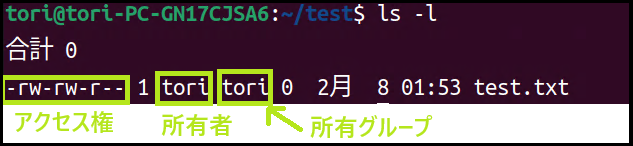
\includegraphics[width=0.8\textwidth]{images/linux-server/5_1-ls-l.png}
  \caption{ls -lの実行結果}
  \label{fig:ls-l}
\end{figure}
\subsection{アクセス権}
Linuxではファイルやディレクトリに対してアクセス権が設定されている。アクセス権は読み取り、書き込み、実行の3つの権限が設定されている。アクセス権は所有者、グループ、その他の3つに設定されている。\\
\begin{hosokubox}{ファイルのアクセス権}
  \begin{itemize}
    \item r : 読み取り権限  ファイルの内容を読み取ることができる
    \item w : 書き込み権限  ファイルの内容を書き込むことができる
    \item x : 実行権限  ファイルを実行することができる
  \end{itemize}
\end{hosokubox}
\begin{hosokubox}{ディレクトリのアクセス権}
  \begin{itemize}
    \item r : 読み取り権限  ディレクトリ内のファイルを表示することができる
    \item w : 書き込み権限  ディレクトリ内にファイルを作成することができる
    \item x : 実行権限  ディレクトリ内に移動することができる
  \end{itemize}
\end{hosokubox}
\begin{johobox}{ls -lで表示される種類について}
  ls -lで表示される先頭の文字はファイルの種類を示している。以下に一部を示す。
  \begin{itemize}
    \item \verb|- : 通常のファイル|
    \item \verb|d : ディレクトリ|
    \item \verb|l : シンボリックリンク|
  \end{itemize}
\end{johobox}
\subsection{パーミッションの変更}
アクセス権の変更にはchmodコマンドを使用する。ただし、アクセス権の変更にはsodo権限が必要である。\\
\begin{commandbox}{chmodコマンドの使用方法}
  \verb|chmod {パーミッション} {ファイル名}|\\
  \verb|chmod {パーミッション} {ディレクトリ名}|
\end{commandbox}
また、アクセス権の変更には記号を用いた方法と数値を用いた方法がある。数値を用いたものは前述しているため、ここでは記号を用いた方法について説明する。
\begin{table}[H]
  \centering
  \caption{chmodコマンドの記号について}
  \begin{tabular}{|c|c|c|} \hline
    対象 & 操作 & 権限 \\ \hline
    u:所有者 & +:追加 & r:読み取り権限 \\
    g:所有グループ & -:削除 & w:書き込み権限 \\
    o:その他ユーザー & =:指定 & x:実行権限 \\
    a:全てのユーザー & & \\ \hline
  \end{tabular}
\end{table}
\begin{hosokubox}{chmodコマンドの使用例}
  \begin{itemize}
    \item \verb|chmod u+x test.txt| : test.txtに所有者に実行権限を追加する
    \item \verb|chmod g-w test.txt| : test.txtに所有グループから書き込み権限を削除する
    \item \verb|chmod o=r test.txt| : test.txtにその他ユーザーに読み取り権限を指定する
    \item \verb|chmod a=rwx test.txt| : test.txtに全てのユーザーに読み取り、書き込み、実行権限を指定する
  \end{itemize}
\end{hosokubox}
\subsection{所有者と所有グループ}
Linuxにおけるファイルやディレクトリは作成したユーザーが所有者・所有グループとなる。しかし、一定以上のサーバー管理となる場合、管理体系などの理由により管理者レベルの高いユーザーに所有権を譲渡する必要がある。その際にchownコマンドを使用する。
\begin{commandbox}{chownコマンドの使用方法}
  \verb|chown {所有者} {ファイル名(ディレクトリ名)}|\\
  \verb|chgrp {所有グループ} {ファイル名(ディレクトリ名)}|
\end{commandbox}
\begin{attentionbox}{chownコマンドの注意点}
  chownコマンドはsudo権限が必要である。また、ファイルやディレクトリの所有者を変更する際は、そのファイルやディレクトリに対して所有者権限を持っている必要がある。
\end{attentionbox}
\section{環境変数}
環境変数は、システム全体で使用される変数である。環境変数はシェルが起動する際に設定され、シェルの終了時に破棄される。環境変数はシェルスクリプトやプログラムから参照することができる。主な環境変数は以下の通りである。\\
\begin{table}[H]
  \centering
  \caption{主な環境変数}
  \begin{tabular}{|c|c|} \hline
    環境変数 & 説明 \\ \hline
    HOME & ユーザーのホームディレクトリのパス \\
    PATH & 実行ファイルの検索パス \\
    USER & ユーザー名 \\
    SHELL & シェルのパス \\
    LANG & 言語設定 \\
    PWD & カレントディレクトリのパス \\
    HISTSIZE & コマンド履歴の最大値 \\
    HISTFILE & コマンド履歴の保存先 \\ \hline
  \end{tabular}
\end{table}
地齋に環境変数を表示するには、echoコマンドを使用する。この時、環境変数名の前に「\texttt{\$}」を付けることで環境変数の値を表示することができる。
\begin{commandbox}{環境変数の表示}
  \verb|$ echo ${環境変数名}|
\end{commandbox}
また、これらの環境変数の値などを一時的に変更したい場合はexportコマンドを使用する。exportコマンドを使用することで、環境変数の値を一時的に変更することができる。
\begin{commandbox}{exportコマンドの使用方法}
  \verb|export {環境変数名}={値}|\\\\
  例:HISTSIZEの値を100に変更する\\
  \verb|$ export HISTSIZE=100|
\end{commandbox}
\begin{hosokubox}{環境変数の値を永続的に変更する}
  環境変数の値を永続的に変更するには、環境変数の設定を行うファイルに環境変数の設定を記述する。環境変数の設定を行うファイルは以下の通りである。変更には「.bash\_profile」や「.bashrc」の末尾にexportコマンドを追記する。
  \begin{itemize}
    \item /etc/profile
    \item /etc/bashrc
    \item \texttt{\~/.bash\_profile}
    \item \texttt{\~/.bashrc}
  \end{itemize}
\end{hosokubox}
\begin{johobox}{環境変数の設定ファイルについて}
  「.bashrc」: システムのログイン時に読み込まれる隠しファイル。\\
  「.bash\_profile」: ユーザーがログインした際に読み込まれるファイル。
\end{johobox}

\section{テキストエディタ}

\section{ネットワーク設定}

\section{ユーザー管理}

\section{SSH}

\section{基本的なサーバー管理}

\section{Webサーバーの構築}

\section{Dockerを使用した環境構築や運用}

\section{終わりに}






\end{document}